Según una antigua leyenda, en un templo en la ciudad de Benarés, India, hay una gran torre con tres varillas de diamante. En una de estas varillas, los monjes han colocado 64 discos de oro, apilados en orden creciente de tamaño desde la base hasta la cima. Los monjes tienen la tarea sagrada de mover todos los discos de la primera varilla a la tercera, siguiendo las reglas  del rompecabezas de las Torres de Hanoi:

\begin{enumerate}
	\item Se puede mover solo un disco a la vez.
	\item Un disco de mayor tamaño no puede estar sobre uno de menor tamaño.
	\item Solo se puede desplazar el disco que esté más arriba de cada varilla.
\end{enumerate}

La leyenda dice que cuando los monjes completen esta tarea, el mundo llegará a su fin. ¿Deberíamos preocuparnos por esto?

\begin{figure}[H]
	\centering
	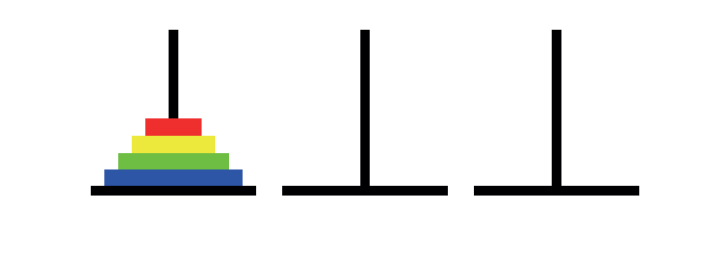
\includegraphics[width=0.45\linewidth]{cp1/hanoi.png}
        \caption{Ejemplo de Torres de Hanoi con 4 discos}
\end{figure}

\textbf{Pista:} Intenta calcular la cantidad de movimientos que los monjes necesitarán para completar su tarea.\\

En esta página (si Etecsa te lo permite) puedes intentar resolverlo con diferentes cantidades de discos: \href{https://www.geogebra.org/m/NqyWJVra}{Torres de Hanoi}.
